\ifSTANDALONE
\section{Prinziptest}
\fi
\ifEMBED
\subsubsection{Aufbaubeschreibung}
    \BLDCcollab
\fi
\ifEMBED
    \begin{wrapfigure}{r}{0.55\textwidth}
       	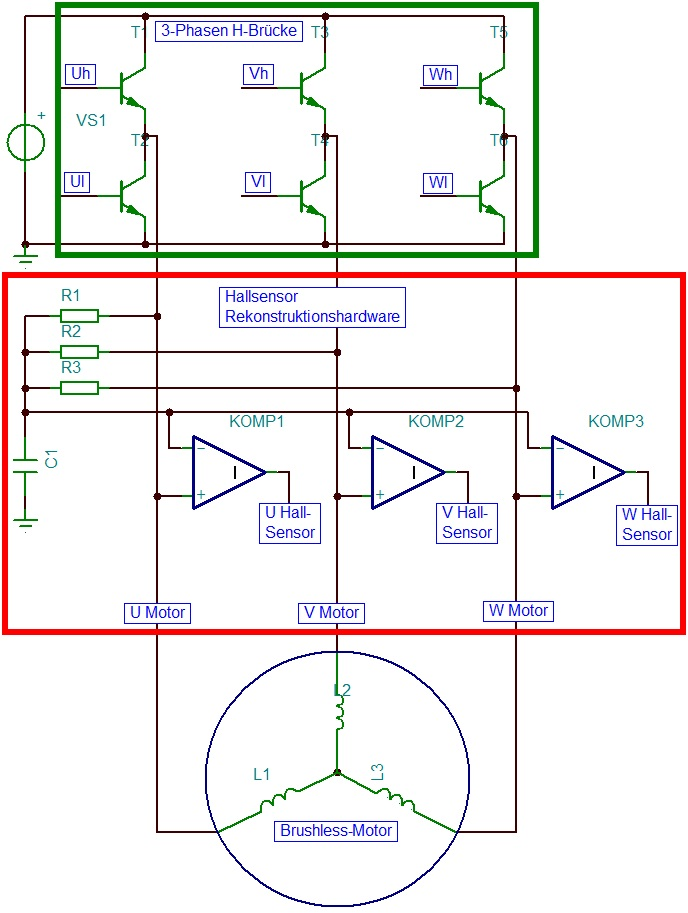
\includegraphics[scale=0.4]{\EtPath/Bilder/MotoransteuerungSchema.jpg}
       	\centering
       	\caption{Schema des Brushless-Versuchsaufbaus}
        \label{abb:MotoransteuerungSchema}
    \end{wrapfigure}
\fi
    Das Schema des Gesamtaufbaus des Tests ist in der Abbildung 
    \ref{abb:MotoransteuerungSchema} ersichtlich. Die 3-Phasen H-Brücke 
    im oberen grünen Rechteck wird direkt vom FPGA \footnote{\textbf{F}ield-\textbf{P}rogrammable \textbf{G}ate \textbf{A}rray} angesteuert. Die Hardware 
    dieser Brücke ermöglicht eine voll galvanisch getrennte Ansteuerung 
    mit 3.3V Logikpegeln. Diese Brücke wurde zur Verfügung gestellt und direkt
    implementiert. Die Rekonstruktion der Hallsensoren-Signale findet im rot 
    markierten Teil des Aufbaus statt. Dieser Part wurde auf einer 
    Laborplatte aufgebaut und gelötet. Die so generierten Signale 
    $U_{Hallsensor}$, $V_{Hallsensor}$, $W_{Hallsensor}$ werden einem FPGA 
    geliefert. Anhand dieser Signale steuert das FPGA die 
    H-Brücken-Transistoren mit den Signalen $U_h$, $U_l$, $V_h$, $V_l$, 
    $W_h$, $W_l$. Die im FPGA enthaltene Konfiguration besteht aus simplen 
    AND-Verknüpfungen, die die anliegenden Signale sehr schnell und 
    effizient verarbeiten können. Auf diese Weise ist es möglich, den Motor sehr 
    schnell anzusteuern.
    \ifSTANDALONE
    \begin{figure}[h!]
    	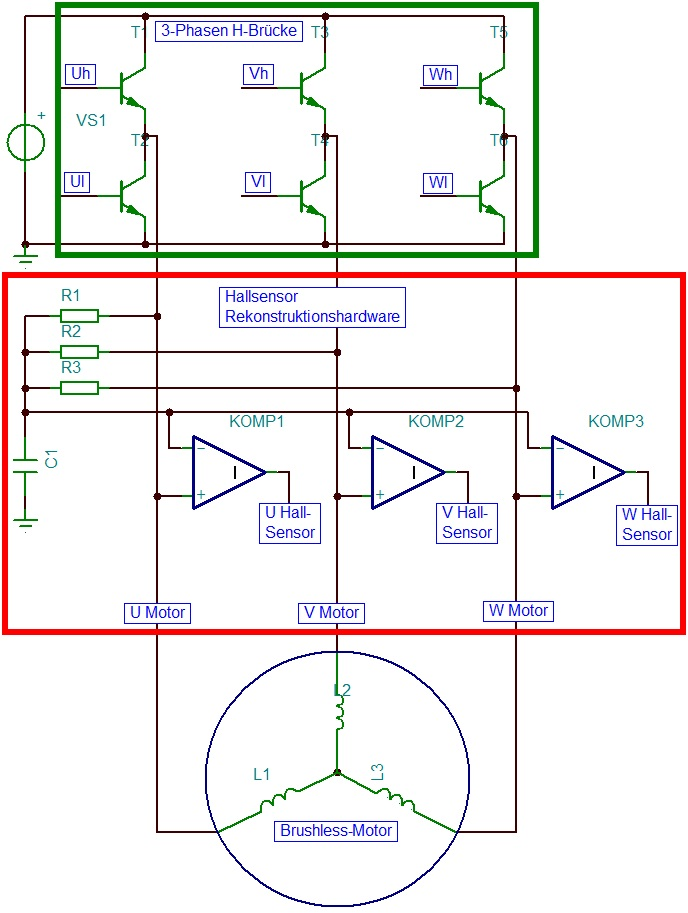
\includegraphics[scale=0.4]{\EtPath/Bilder/MotoransteuerungSchema.jpg}
       	\centering
       	\caption{Schema des Brushless-Versuchsaufbaus}
        \label{abb:MotoransteuerungSchema}
    \end{figure}
    \fi
    In der Abbildung \ref{abb:MessplatzAufbau} ist der gesamte Aufbau 
    abgebildet. Man beachte die markierten Felder. Am linken unteren Rand 
    ist der Motor befestigt. In der Mitte des Bildes ist die Hardware zur Rekonstruktion der Hallsensoren-Signale.
    Die generierten Signale werden dem FPGA in der unteren linken Ecke zugeführt. Diese 
    Signale werden logisch verknüpft und danach die sechs Signale 
    generiert, um die H-Brücke in der rechten oberen Hälfte anzusteuern. 
    Die H-Brücken wiederum treiben den Motor an.
    \begin{figure}[h!]
    %\vspace{-16pt}
       	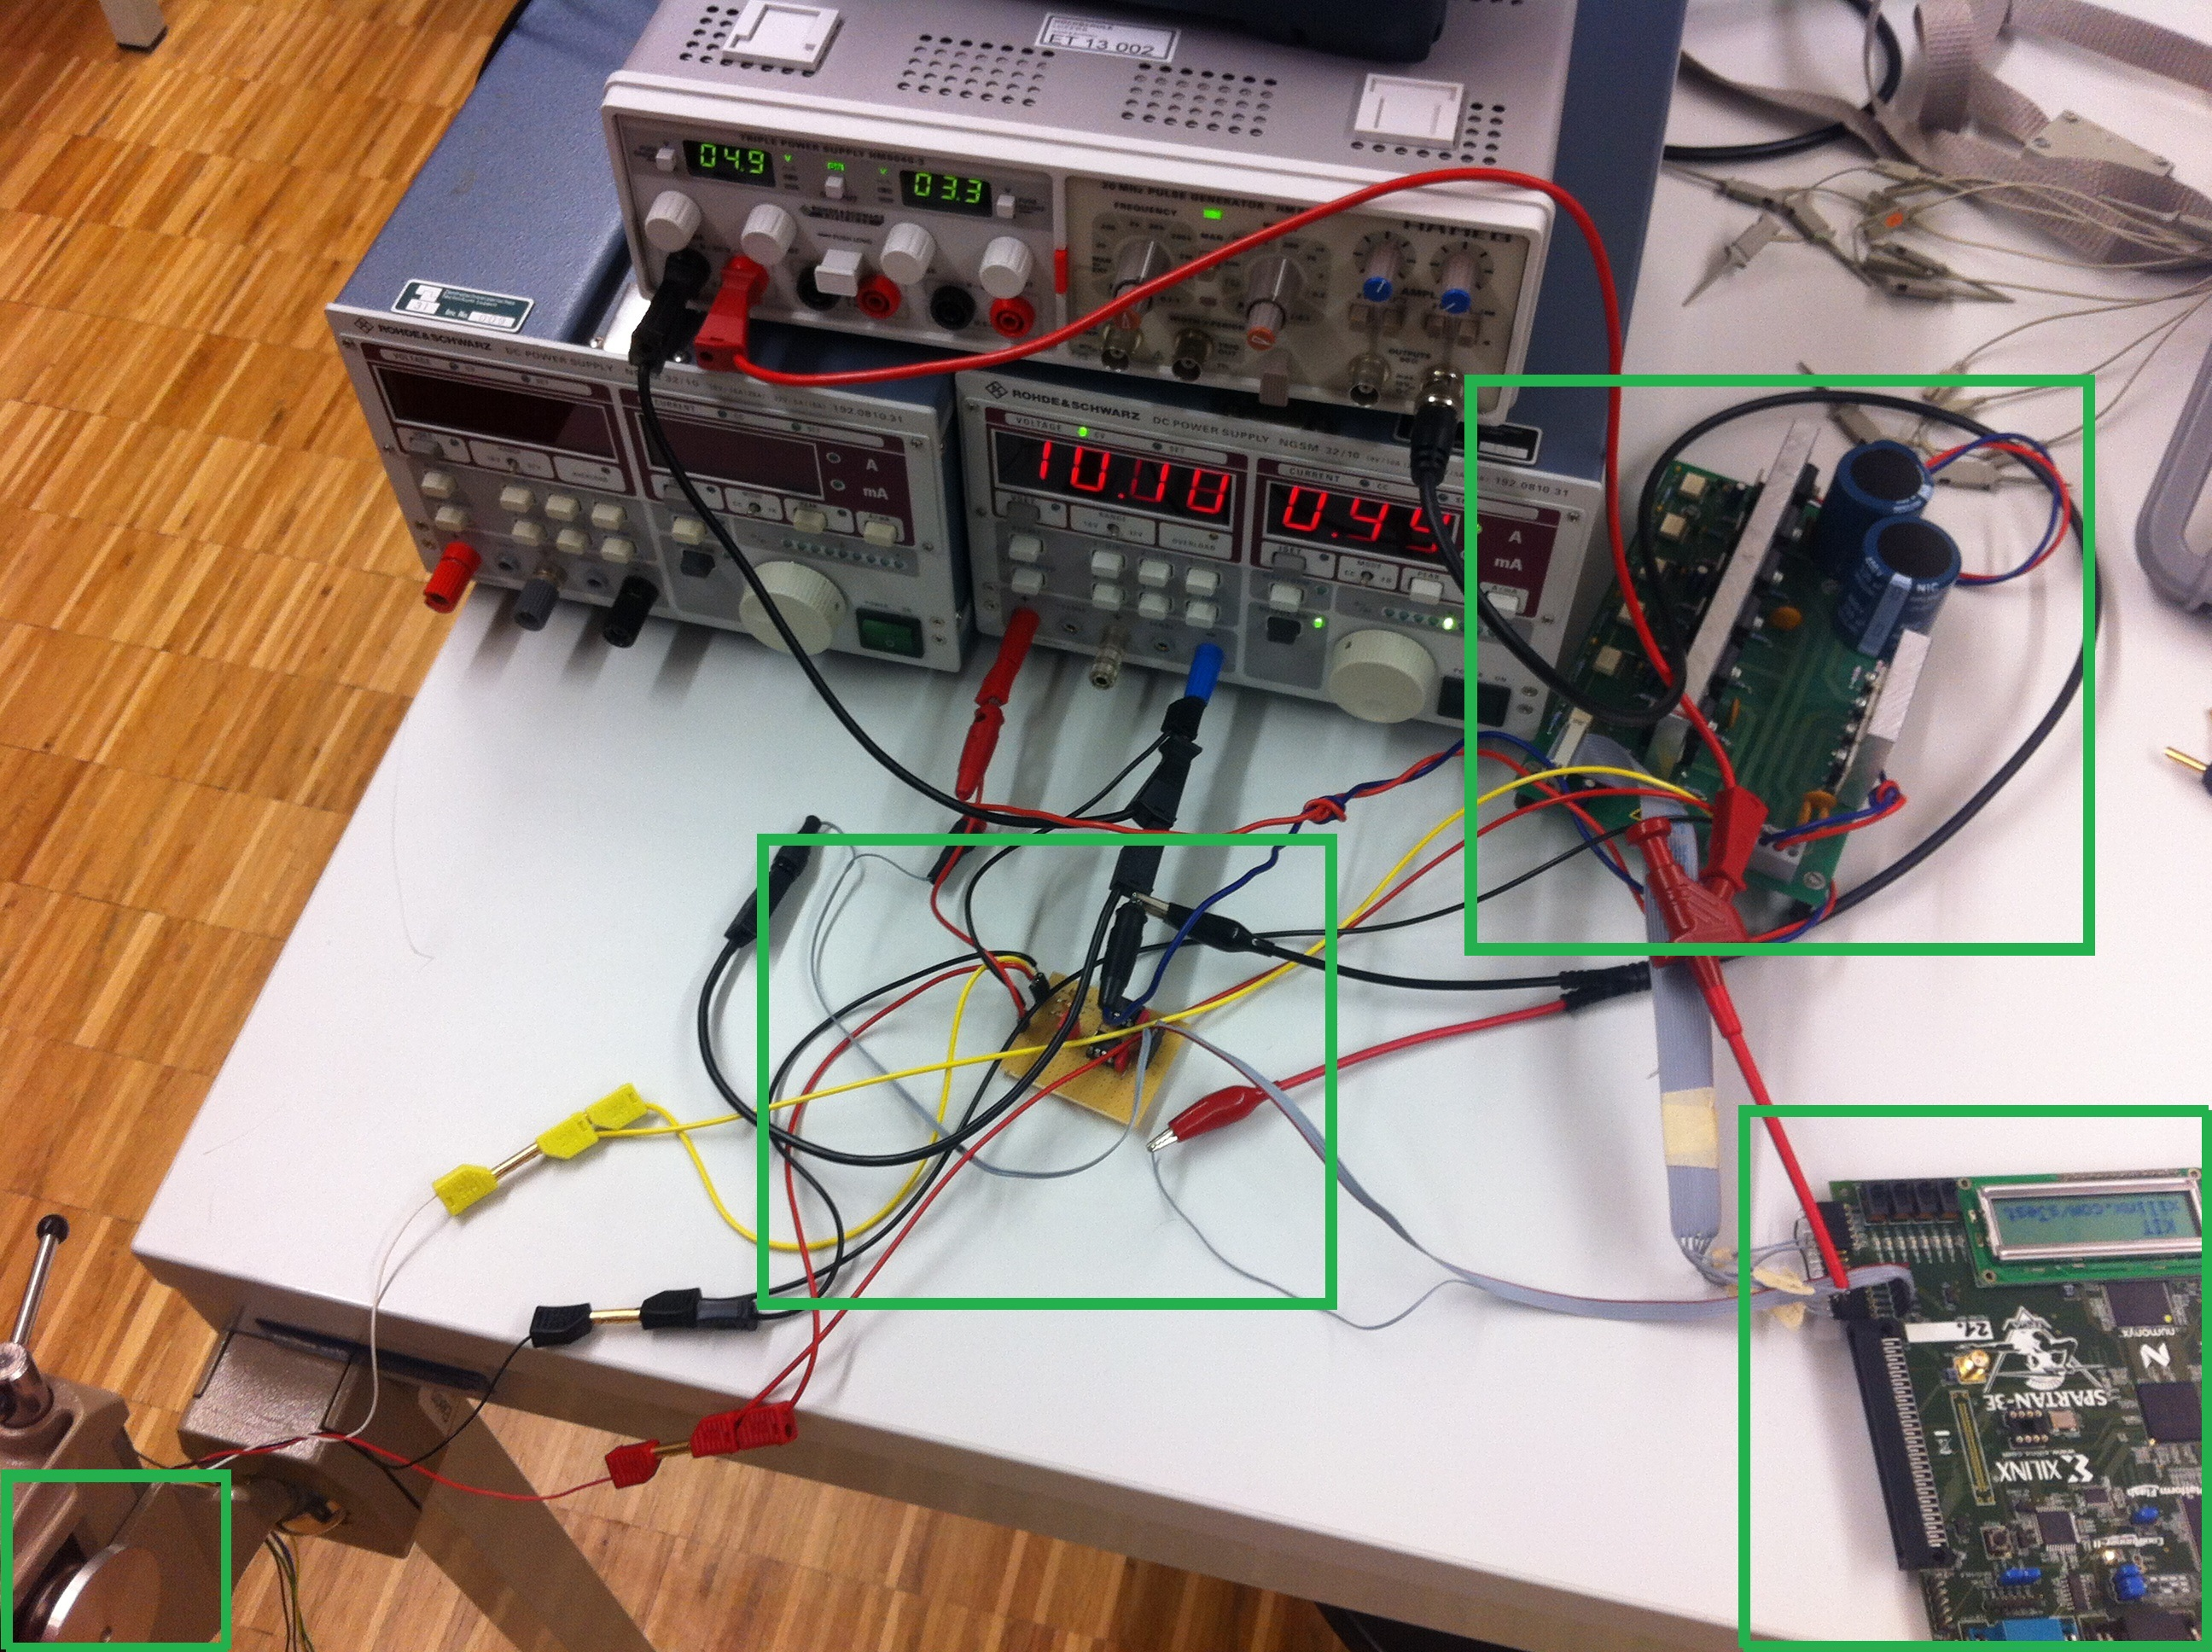
\includegraphics[scale=0.14]{\EtPath/Bilder/MessplatzAufbau.jpg}
       	\centering
       	\caption{Testaufbau} 
        \label{abb:MessplatzAufbau}
    %\vspace{-10pt}
    \end{figure}
    Die im FPGA enthaltene Logik basiert auf der Wahrheitstabelle, die in 
    Abbildung \ref{abb:WahrheitstabelleAnsteuerung} abgebildet ist.

\ifSTANDALONE
\subsection{Messmittel}
\fi
\ifEMBED
\subsubsection{Messmittel}
\fi
    \begin{table}[h!]
        \centering
        \begin{tabular}{lll}
            \rowcolor{gray}
            Gerät &
                Typ &
                Nummer \\
            Speisegerät & 
                Rohde \& Schwarz NGSM 32/10 &
                Inv.-Nr. 009 \\
            Oszilloskop &
                Agilent MSO6052A &
                Inv.-Nr. 44; S/N: MY44001903 \\
            Mainframe &
                Hameg HM8001-2 &
                SN: 059520046 \\
            Speisegerät &
                Hameg HM8040-3 &
                SN: 015405014 \\
            Pulsgenerator &
                Hameg HM8035 &
                Inv.-Nr. 44 \\
        \end{tabular}
        \caption{Messmittel des Versuchsaufbaus}
    \end{table}
